\documentclass[]{jlreq}

\usepackage{graphicx}
\usepackage[pdfencoding=auto]{hyperref}
\usepackage{amsmath,amssymb,amsthm}
\theoremstyle{definition}
\usepackage{bm}
\usepackage{booktabs}
%\usepackage{subfig}
\usepackage{pifont}
\usepackage{url}
\usepackage{cite}
\usepackage{ulem}
\usepackage{siunitx}
\usepackage{float}
\usepackage{tcolorbox}
\tcbuselibrary{breakable}
\usepackage{cancel}
\usepackage{color}
\renewcommand{\CancelColor}{\color{red}}
\renewcommand{\abstractname}{}

\usepackage{tikz}
\usetikzlibrary{shadows}
\usetikzlibrary{calc}
%\usepackage{circuitikz}

\usepackage{luatexja-fontspec}
\renewcommand{\figurename}{Fig.~}
\renewcommand{\tablename}{Table~}

\hypersetup{
  colorlinks=false, % リンクに色をつけない設定
  %bookmarks=true, % 以下ブックマークに関する設定
  bookmarksnumbered=true,
  pdfborder={0 0 0},
  bookmarkstype=toc
}

\begin{document}
\title{Time-domain and Frequency-domain Signals}
\author{吉本伸一}
\maketitle
\tableofcontents
\clearpage

\section{Fourier級数展開}
周期が$T_0$の周期関数$f(t)$をFourier級数展開すると
%
\begin{equation}
  f(t) = \sum_{n=-\infty}^{\infty} c_n e^{j n \omega_0 t}
  \label{fourier_series}
\end{equation}
%
\begin{equation}
  c_n = \frac{1}{T_0} \int_{-T_0/2}^{T_0/2} f(t) e^{- j n \omega_0 t} dt \; (n = 0, \pm 1, \pm 2, \pm 3, \dots)
  \label{fourier_coef}
\end{equation}
%
ただし、$\omega_0 = 2\pi/T_0$とおいた。
%
\section{Fourier変換}
\begin{equation}
  \mathcal{F}[f(t)] = F(\omega) = \int_{-\infty}^{\infty} f(t) e^{-j\omega t} dt
\end{equation}
\begin{equation}
  \mathcal{F}^{-1}[F(\omega)] = f(t) = \frac{1}{2\pi}\int_{-\infty}^{\infty} F(\omega) e^{j\omega t} d\omega
\end{equation}

\section{デルタ関数}
\begin{equation}
  \int_{-\infty}^{\infty} \delta (x) dx = 1
\end{equation}
%
\begin{equation}
  \int_{-\infty}^{\infty} f(x) \delta (x) dx = f(0)
\end{equation}
%
\begin{equation}
  \int_{-\infty}^{\infty} f(x) \delta (x - a) dx = f(a)
\end{equation}
%
\section{デルタ関数のFourier変換}
%
\begin{equation}
  \mathcal{F}[\delta (t)] = \int_{-\infty}^{\infty} \delta (t) e^{- j \omega t} dt = 1
  \label{fd1}
\end{equation}
%
\begin{equation}
  \mathcal{F}[\delta (t - t_0)] = \int_{-\infty}^{\infty} \delta (t - t_0) e^{- j \omega t} dt = e^{-j \omega t_0}
  \label{fd2}
\end{equation}
%
\begin{equation}
  \mathcal{F}^{-1} [\delta(\omega)] = \frac{1}{2\pi}\int_{-\infty}^{\infty} \delta (\omega) e^{j \omega t } d\omega = \frac{1}{2\pi}
\end{equation}
%
したがって、
%
\begin{equation}
  \mathcal{F}[1] = 2\pi\delta(\omega)
  \label{f1}
\end{equation}
%
\section{ポアソン和公式}

$F(\omega) = \mathcal{F}[f(t)]$とした時、

\begin{equation}
  \sum_{n=-\infty}^{\infty} f(\alpha n) = \frac{1}{\alpha} \sum_{n=-\infty}^{\infty} F\left( \frac{2 \pi n}{\alpha}\right)
\end{equation}
%
が成り立つ。これをポアソン和公式 (Poisson summation formula) という。
%
\begin{proof}
  (\ref{fd2})より
  \begin{equation}
    \sum_{n=-\infty}^{\infty} f(\alpha n) = \sum_{n=-\infty}^{\infty}\int_{-\infty}^{\infty} f(t) \delta(t - \alpha n) dt
  \end{equation}
  %
  $\sum \delta(t - \alpha n)$は、周期$\alpha$の周期関数なのでフーリエ級数展開でき、区間$[-\alpha/2, \alpha/2]$において$\delta(t-\alpha n)$は$\delta(t)$とみなせるので、$\omega_0 = 2\pi/\alpha$とおくと(\ref{fourier_series}), (\ref{fourier_coef})より
  %
  \begin{align}
    \sum_{n=-\infty}^{\infty}\delta(t - \alpha n) 
    &= \sum_{n=-\infty}^{\infty} \frac{1}{\alpha} \left[ \int_{-\alpha/2}^{\alpha/2} \delta(t) e^{-j n\omega_0 t} dt \right] e^{j n \omega_0 t} \\
    &= \frac{1}{\alpha} \sum_{n=-\infty}^{\infty} e^{j n\omega_0 t} = \frac{1}{\alpha} \sum_{n=-\infty}^{\infty} e^{-j n\omega_0 t} 
  \end{align}
  %
  したがって、
  %
  \begin{align}
    \sum_{n=-\infty}^{\infty} f(\alpha n) &=\frac{1}{\alpha} \sum_{n=-\infty}^{\infty} \int_{-\infty}^{\infty} f(t) e^{-j n \omega_0 t} dt \notag\\
      &= \frac{1}{\alpha} \sum_{n=-\infty}^{\infty}F(n\omega_0) 
      = \frac{1}{\alpha} \sum_{n=-\infty}^{\infty} F\left( \frac{2 \pi n}{\alpha}\right) \notag
  \end{align}
\end{proof}
%
\section{Single-bunch Spectrum}
リングに1個のバンチが周期が$T_0$で周回している時、ビームの信号は、
%
\begin{equation}
  i(t) = \sum_{n=-\infty}^{\infty} \delta (t - n T_0 ) 
\end{equation}
%
のように表すことができる。ここで、$i(t)$をフーリエ変換すると、
%
\begin{align}
  I(\omega) &= \int_{-\infty}^{\infty} i(t) e^{-j \omega t} dt
    = \sum_{n=-\infty}^{\infty} \int_{-\infty}^{\infty} \delta (t - n T_0 ) e^{-j \omega t} dt \notag \\ 
    &= \sum_{n=-\infty}^{\infty} e^{-j\omega n T_0} = \sum_{n=-\infty}^{\infty} e^{-j 2\pi n \frac{\omega}{\omega_0}}
\end{align}
%
ただし、$T_0 = 2\pi / \omega_0$とした。ここで、$f(t) = e^{-j\omega t}, \alpha = 2\pi /\omega_0$として、ポワソン和公式を使うと、
%
\begin{align}
  I(\omega) &= \sum_{n=-\infty}^{\infty} e^{-j 2\pi n \frac{\omega}{\omega_0}} = \sum_{n=-\infty}^{\infty} f(\alpha n)\notag \\
    &= \frac{1}{\alpha} \sum_{n=-\infty}^{\infty} F\left( \frac{2 \pi n}{\alpha}\right) 
    = \frac{\omega_0}{2\pi} \sum_{n=-\infty}^{\infty} F(n \omega_0) \notag \\
    &= \frac{\omega_0}{2\pi} \sum_{n=-\infty}^{\infty} \int_{-\infty}^{\infty} f(t) e^{-j n \omega_0 t} dt \notag \\
    &= \frac{\omega_0}{2\pi} \sum_{n=-\infty}^{\infty} \int_{-\infty}^{\infty} e^{-j (\omega + n \omega_0) t} dt \notag \\
    &= \omega_0 \sum_{n=-\infty}^{\infty} \delta(\omega + n \omega_0) \qquad (\because (\ref{f1})) \notag \\
    &= \omega_0 \sum_{n=-\infty}^{\infty} \delta(\omega - n \omega_0)
\end{align}
%
これより、周期$T_0$で周回するバンチのスペクトルをスペアナなどで観測すると、周回周波数$\omega_0$毎にピークを持つ信号が観測されることがわかる。
%
\begin{figure}[hbt]
  \begin{center}
    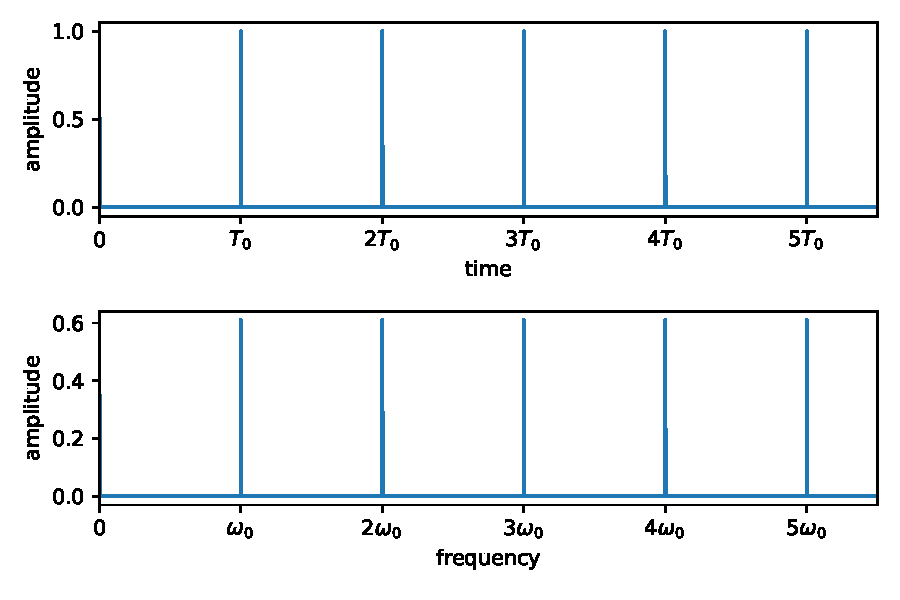
\includegraphics[width=12cm,clip]{single_bunch.pdf}
    \caption{単バンチのビーム信号のスペクトル.}
   \label{single_bunch}
  \end{center}
\end{figure}
%
\section{Multi-bunch Spectrum}
リングにM個のバンチが均等に配置されている場合、ビームの信号は
%
\begin{equation}
  i(t) = \sum_{k=-\infty}^{\infty} \sum_{n=0}^{M-1}\delta (t - k T_0 -n T_0 / M)
\end{equation}
%
と表すことができる。先程と同様にフーリエ変換すると、
%
\begin{align}
  I(\omega) &= \int_{-\infty}^{\infty} i(t) e^{-j \omega t} dt\notag\\
    & = \sum_{k=-\infty}^{\infty} \sum_{n=-\infty}^{\infty} \int_{-\infty}^{\infty} \delta (t - k T_0 - n T_0/M) e^{-j \omega t} dt \notag \\ 
    &= \sum_{k=-\infty}^{\infty} \sum_{n=-\infty}^{\infty} e^{-j\omega (k T_0 + n T_0 / M)} \\
    &= \sum_{n=-\infty}^{\infty} e^{-j 2\pi n \frac{\omega}{\omega_0}}
\end{align}
%
ただし、$T_0 = 2\pi / \omega_0$とした。ここで、$f(t) = e^{-j\omega t}, \alpha = 2\pi /\omega_0$として、ポワソン和公式を使うと、
%




くし型関数と同様に考えると、$f(t)$は周期$T_0/M$の周期関数で、区間$[-T_0/2M, T_0/2M]$においては$f(t)$は$\delta(t)$とみなせるから
%
%
\begin{align}
  f(t) &= \sum_{n = -\infty}^{\infty} \frac{M}{T_0} \left[\int_{-T_0/2M}^{T_0/2M}\delta (t) e^{-j n M \omega_0 t} dt\right] 
  e^{j n M \omega_0 t} \\
              &= \frac{M}{T_0} \sum_{n = -\infty}^{\infty} e^{j n M \omega_0 t} 
\end{align}
%
したがって、
%
\begin{align}
  \mathcal{F}[f(t)] &= \mathcal{F}\left[\frac{M}{T_0} \sum_{n = -\infty}^{\infty} e^{j n M \omega_0 t}\right] \\ 
      & = \frac{M}{T_0} \sum_{n = -\infty}^{\infty} \mathcal{F}[\mathcal{F}^{-1}[2\pi \delta(\omega - n M \omega_0)]] \\ 
      & = \frac{2 \pi M}{T_0} \sum_{n = -\infty}^{\infty} \delta(\omega - n M \omega_0)\\ 
      &= M \omega_0 \sum_{n = -\infty}^{\infty} \delta(\omega - n M \omega_0)
\end{align}
%
\begin{figure}[hbt]
  \begin{center}
    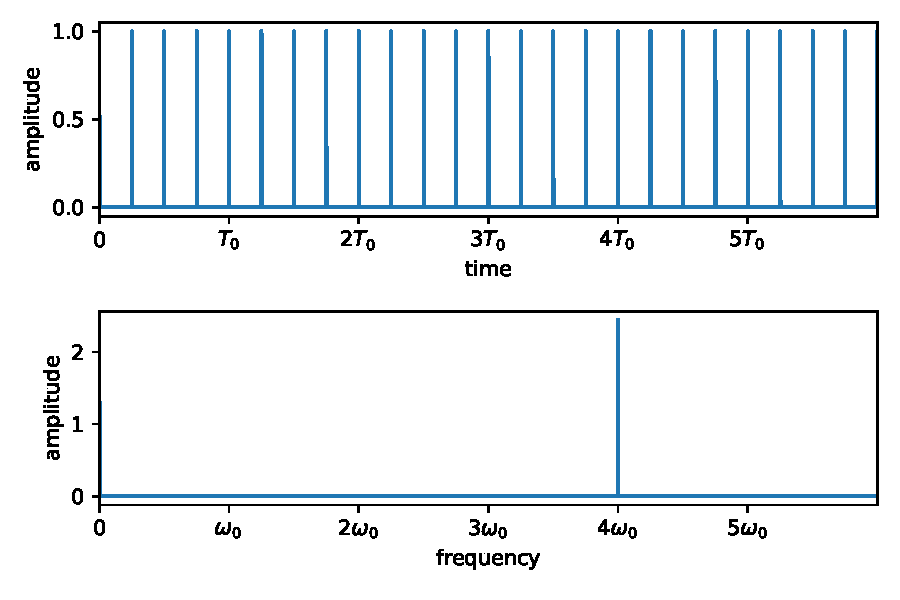
\includegraphics[width=12cm,clip]{multi_bunch.pdf}
    \caption{多バンチのビーム信号のスペクトル.}
   \label{multi_bunch}
  \end{center}
\end{figure}
%
\section{Synchrotron oscillation}
\begin{equation}
  i(t) = \sum_{n=-\infty}^{\infty}\delta[t - n T_0 - \tau_a \cos(\omega_s n T_0 + \phi)]
\end{equation}
%
\begin{align}
  F(\omega) &= \int_{-\infty}^{\infty} i(t) e^{-j\omega t} dt \\
  &= \sum_{n = -\infty}^{\infty} e^{-j\omega\{n T_0 + \tau_a \cos(\omega_s n T_0 + \phi)\}} \\
  &= \sum_{n = -\infty}^{\infty} \left[ e^{-j\omega n T_0 }+ e^{-j \omega \tau_a \cos(\omega_s n T_0 + \phi)} \right]
\end{align}
%
ここで、
%
\begin{equation}
  e^{jz\cos\theta} = \sum_{k = -\infty}^{\infty} j^k J_k(z) e^{j k \theta}
\end{equation}
%
という関係を使うと(ただし、$J_n$はベッセル関数)
%
\begin{align}
  F(\omega) &= \sum_{k = -\infty}^{\infty} (-j)^k J_k(\omega \tau_a) e^{j k \phi} \sum_{n = -\infty}^{\infty} e^{-j (\omega + k \omega_s) n T_0} \\
    &= \omega_0 \sum_{k = -\infty}^{\infty} (-j)^k J_k(\omega \tau_a) e^{j k \phi} \sum_{n = -\infty}^{\infty} \delta(\omega + k\omega_s - n \omega_0)
\end{align}
%
\begin{thebibliography}{9}
  \bibitem{Hiramatsu}
  平松成範, 加速器のビームモニター (Beam Instrumentaion for Accelerrators), KEK Internal 2004-4 A.
\end{thebibliography}
%
\end{document}